\documentclass[
    aps,
    prd,
    reprint,
    onecolumn,
    %groupedaddress,
    superscriptaddress,
    linenumbers,
    nolongbibliography,
    nobibnotes,
    nofootinbib,
    %floatfix,
]{revtex4-2}

\bibliographystyle{apsrev4-2}

\usepackage[dvipsnames, usenames]{xcolor}
\definecolor{linkcolor}{rgb}{0.1, 0.5, 0.7}

\usepackage[
colorlinks=true,
linkcolor=linkcolor,
citecolor=linkcolor,
filecolor=linkcolor,
urlcolor=linkcolor,
pdfusetitle,
]{hyperref}

\usepackage{amssymb}
\usepackage{amsmath}
\usepackage{physics}
\usepackage{orcidlink}

\usepackage{fontawesome}

\newcommand{\comment}[1]{}
\newcommand{\red}[1]{{\color{Red} #1}}
\newcommand{\todo}[1]{{\color{red}TODO:}{\color{blue}#1}}
\newcommand{\citeme}[1]{{\color{red}CITEME:}{\color{blue}#1}}




\begin{document}


\title{Notes for 14 Nov 25}

\date{\today}

\maketitle


\section{Agenda/Notes}

\begin{itemize}
    \item Big picture -- what can we think of outside the supernova engine that could give rise to the peak we see in the population?
    \begin{itemize}
        \item Tilts are just hard to measure with GWs and we got unlucky? \faicon{wrench}
        \item Lack of mass transfer b/t supernovae \checkmark
        \item Off-axis kicks \faicon{circle}
        \item three-body interactions (out-of-scope)
    \end{itemize}
    \item Population Synthesis
    \begin{itemize}
        \item \texttt{POSYDON} already runs by neglecting to re-align first-born compact-object with orbit during mass transfer b/c it assumes Eddington-limited accretion
        \item So I think this is already the most conservative case for what we want to study -- not even re-alignment give us peaks away from $\cos \theta = \pm 1$
        \begin{figure}[h]
            \centering
            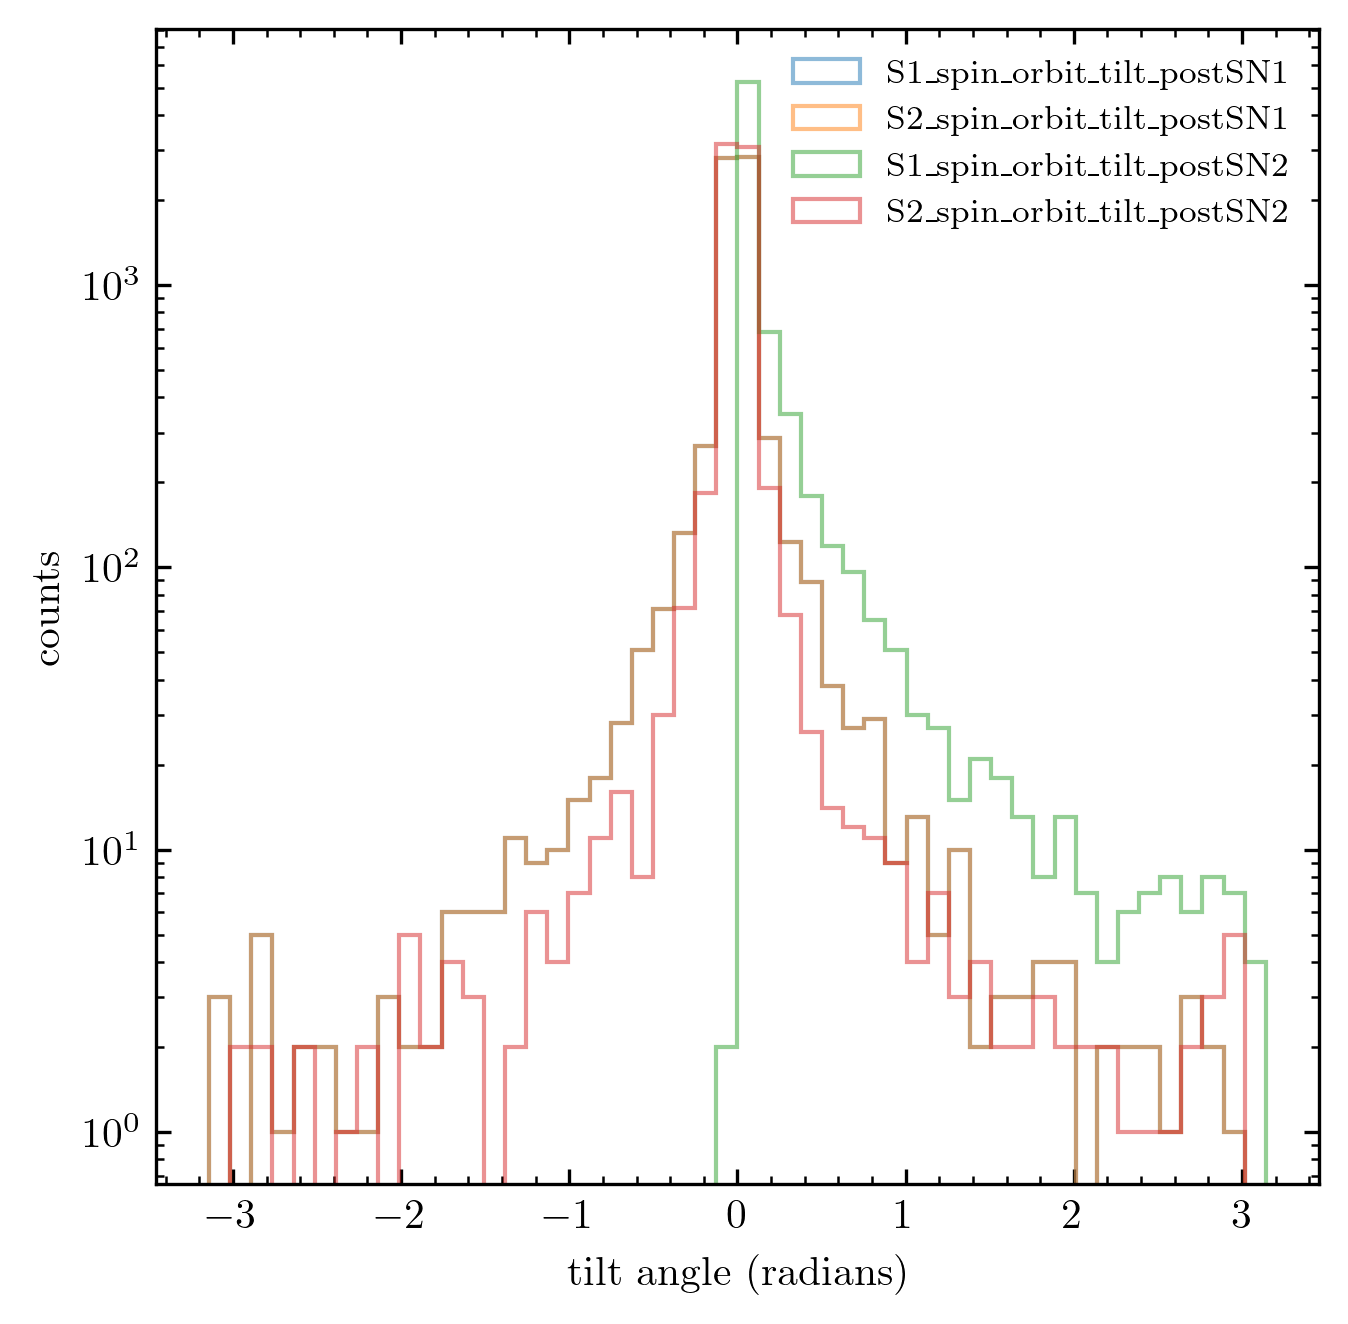
\includegraphics[width=0.5\linewidth]{./figures/BBH_spin_tilts.png}
            \caption{Caption}
            \label{fig:placeholder}
        \end{figure}
        \item So that *might* be minimum-viable hardcore pop. synth., actually? We can use it to guide our mock study and population inference---in terms of peakiness and correlations. Also timescales of evolution from BH+BH formation to merger for precession-evolution calculation.
        \item If we want to study the effects of, e.g., off-axis kicks, we could go to another pop. synth code. I looked at cosmic, but its written in \texttt{FORTRAN}...
    \end{itemize}
    \item Mock Catalog
    \begin{itemize}
        \item \todo{dump other plots of distribution here}
        \item Three challenges:
        \begin{itemize}
            \item Limited compute (at most a few hundred CPUs at a time, can only run for 18 hrs at a time, re-queues of up to a week at a time)
            \item We'll need $\sim 10^4$ PE runs to be able to \textit{independently} re-sample to distributions of interest
            \item \textsc{IMRPhenomXPHM} runs will likely require very expensive re-runs (heterodyned -> full likelihood)
        \end{itemize}
        \item Let's make it easy on ourselves by running with \textsc{IMRPhenomXP}.
        \item \textbf{Next step}: run a limited catalog of 70 sources with $\rho > 15$ and isotropic spin-tilts. \textit{Select} with \textsc{IMRPhenomXP} but run PE with both \textsc{IMRPhenomXP} and \textsc{IMRPhenomXPHM} -- compare measurement uncertainties at single-event and catalog level.
        \begin{itemize}
            \item Unless we see noticeable differences in our ability to measure spin tilts (esp. at pop level), we'll use \textsc{IMRPhenomXP}
        \end{itemize}
        \item \textbf{Population:} do some kind of heuristic fit to pop. synth. cosine tilt distributions and fit a ``low kicks" and ``high kicks" case (extremely peaky vs. somewhat less peaky)
    \end{itemize}

    \item Miscellany
    \begin{itemize}
        \item How does \texttt{Posydon} handle core-collapse for stellar mergers?
        \item Started PE runs with \textsc{IMRPhenomXPHM} but they are taking a while!
        \begin{itemize}
            \item Initial test set of $10^3$ PE runs drawn from isotropic spin tilt distribution
            \item I previously thought \textsc{IMRPhenomXPHM} was the bottleneck---but likelihood evaluation times are $\sim 2 - 6 \times 10^{-3}$\,s (w/ relative binning likelihood).
            If we assume we need $10^7 - 10^8$ likelihood evaluations, each run should take $\lesssim 1$\,week.
            \item Comparable (I think) to previous mock catalog with \textsc{IMRPhenomXP} (though that was sped up by using 10 CPUs per run instead of 1)
            \item \textbf{The real problem is that my runs are stuck in the queue for up to a week each!}
        \end{itemize}
    \end{itemize}
\end{itemize}

\end{document}
